\chapter{Application: Path Guiding}
\label{ch:application_pg}


\section{Path Guiding}
\label{sec:path_guiding}
The idea behind importance sampling is to let the sampling density be proportional to the integrand
to get as small as possible variance in the result or image in our use case.
Normally we can use the BRDF and the direct illumination to create two sampling distributions,
but one important part is that the indirect illumination is not known beforehand and therefore can't be used easily.
That's exactly what path guiding was created for.
It learns the incident radiance and builds a distribution based on this.
This distribution is then used to create a new image from scratch to create a better distribution
until the final iteration yields the image after combining all iterations weighted by their inverse variance~\cite{Vorba_2019}.
During rendering the distribution can be normally used in MIS
where their created pdf is proportional to the reflected light $ L_r(x, \omega_i) $ from the rendering Equation~\ref{eq:rendering_equation}
and therefore the combined pdf matches the integrand closer.


\section{MIS Compensation in Path Guiding}
\label{sec:misc_path_guiding}
In this section we will show you the results from~\cite[Section~8-9]{Karlik2019}
where they computed the full global illumination instead of only the unoccluded direct illumination as in Section~\ref{sec:ibl_setup} by using this integral:
$$ L(x, \omega_o) = \int_{H(n)} L_G(x, \omega_i)\rho(x, \omega_o, \omega_i) |\omega_i \cdot n|_+ d\omega_i. $$
The difference to the integral in~\ref{eq:ibl_render_equation} is that the emission from the environment map $ L_I(\omega_i) $
is replaced by the total radiance $ L_G(x, \omega_i) $ contributing to a point $ x $ on the surface from direction $ \omega_i $.

Path guiding usually used the BRDF-cosine product and the learned global illumination as the pdfs for MIS.
Karl\'ik et al. used the algorithm presented by M\"uller et al.~\cite{mueller2017}
where the approximation of $ L_G(x, \omega_i) $ is stored in a 5D spatio-directional tree structure.
Because this structure is tabulated it can be easily modified for their purposes,
but it also covers incoming directions and surface positions which makes it larger in size compared to the tabulated map used in Section~\ref{sec:misc_ibl}.
They decided to only implement the normal-independent solution
as the MIS compensation and the normal-dependent pdf would require the table to also cover outgoing directions and normals, respectively.
The general formula for the normal-independent pdf is now:
$$ p_G^{ni}(x, \omega_i) = \frac{1}{b_{ni}} \max \{ 0, L_G(x, \omega_i) - 2 (1 - c_G) \bar{L}_G(x) \}. $$
$ \bar{L}_G(x) $ is the mean radiance arriving at surface position $ x $ and $ b_{ni} $ ensures that it integrates to one.\\
The data structure of M\"uller et al.~\cite{mueller2017} first descends the binary tree that divides 3D space to find the leaf in which position $ x $ is located.
This leaf stores a quad tree which resembles the 2D direction domain in which each leaf $ Q $ holds the estimate of the total radiance $ \hat{L}_G(x, Q) $ coming from that direction $ Q $.
The leaf quad $ Q_i $ is selected proportional to the estimate and the directions in $ Q_i $ are sampled uniformly to get $ \omega_i $.
The final formulation is then archived by integrating $ p_G^{ni}(x, \omega_i) $ over all directions $ \omega_i $ in $ Q_i $ to get
\begin{equation}
    \label{eq:pg_ni}
    p_G^{ni}(x, Q_i) = \frac{1}{b'_{ni}} \max \{ 0, \hat{L}_G(x, Q_i) - 2 (1 - c_G) |Q_i| \sum_k \hat{L}_G(x, Q_k) \}
\end{equation}
with the area of the leaf quad $ Q_i $ represented as $ |Q_i| $.

Since the algorithm of M\"uller et al.~\cite{mueller2017} works iteratively they applied~\ref{eq:pg_ni} at the beginning of each iteration over all quad trees to modify the pdf.
Their modification results in variance reduction and also shorter paths
as they hit the light source earlier which further reduced rendering times by 7\% according to their work~\cite[Section~9]{Karlik2019}.
In Figure~\ref{fig:path_scenes} you can see that using this technique also reduced variance in complex scenarios like specular-diffuse-specular paths as in the Pool scene.
The improvement is not as large as in the IBL example since indirect illumination is generally of lower contrast,
but it still reduced variance and shortens render times while they couldn't observe any failure cases.

\begin{figure}[h]
    \centering
    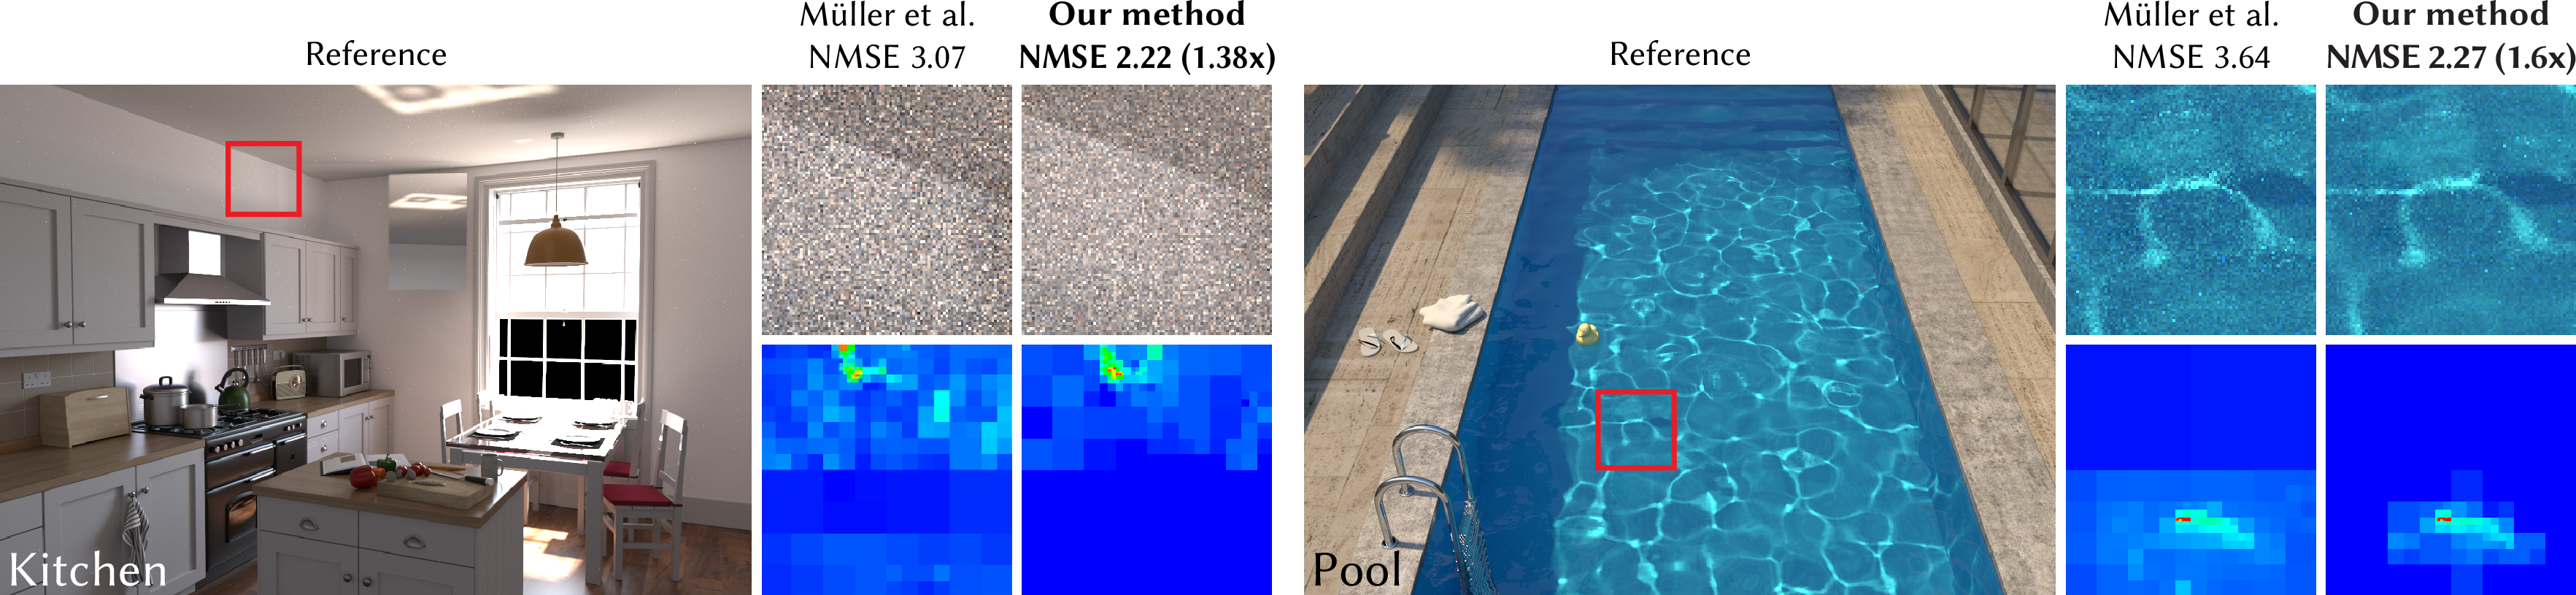
\includegraphics[width=\textwidth]{images/pg_scenes.png}
    \caption{Comparison of the algorithm from M\"uller et al.~\cite{mueller2017} and the practical normal-independent solution form~\cite{Karlik2019} applied to that algorithm.
    Renders are created in equal time (150s).
    The bottom row shows a false color visualization of the quad-tree guiding pdf from the center position of the inset above it.
    \cite[Figure~10]{Karlik2019}}
    \label{fig:path_scenes}
\end{figure}